\chapter{Planificación y presupuesto}

La metodología de trabajo utilizada a la hora de desarrollar este proyecto está basada en la creación y prueba de prototipos de manera iterativa, ya que al tratarse de un proyecto de desarrollo de hardware principalmente se ha considerado que esta es la mejor manera de comprobar si el prototipo funciona como se esperaba o existe algún tipo de fallo el cuál puede ser arreglado en el siguiente prototipo. Además dados los escasos conocimientos iniciales que se tenían en electrónica y electricidad este esquema de desarrollo ha permitido aprender de manera más gradual y práctica. Esta metodología de trabajo se verá reflejada en la planificación propuesta inicialmente que se especificará a continuación así como una estimación del coste total del proyecto.

\section{Planificación del trabajo}
Esta planificación fue realizada cuando aún no se había empezado a trabajar en el proyecto por lo tanto algunos de estos plazos finalmente no se han cumplido tal y como se esperaba.

\begin{itemize}
	\item\textbf{Módulo hardware:}
		\begin{itemize}
			\item Reunión con la persona interesada en el proyecto 16/02/2017 - 16/02/2017. 
			\item Investigación de todas las alternativas existentes para llevar a cabo esta parte del proyecto 16/02/2017- 22/02/2017.
			\item Adquirir todos los componentes necesarios para esta parte comparando los precios y el producto en si que ofrecía cada tienda 22/02/2017 - 23/02/2017.
			\item Diseño de prototipos 23/02/2017 - 17/03/2017.
			\item Montaje de los prototipos diseñados con realización de pruebas para comprobar su correcto funcionamiento 1/03/2017 - 14/04/2017.
			\item Diseño de las placas de las versiones finales 14/04/2017 - 21/04/2017.
			\item Soldar las versiones finales en una PCB 21/04/2017 - 28/04/2017.
			\item Probar las versiones finales 28/04/2017 - 03/05/2017.
			\item Diseño de cajas donde irá colocada la pcb y el resto de componentes de la versión final 03/05/2017 - 04/05/2017.
			\item Montaje de las cajas 04/05/2017 - 05/05/2017.
		\end{itemize}
	\item\textbf{Módulo firmware:}
		\begin{itemize}
			\item Reunión con la persona interesada en el proyecto 16/02/2107 - 16/02/2017. 
			\item Investigación de todas las alternativas existentes para llevar a cabo esta parte del proyecto 16/02/2017- 22/02/2017.
			\item Desarrollo de toda la parte firmware que se subirá a la placa ESP8266 1/03/2017 - 02/06/2017.
			\item Pruebas 02/06/2017 - 09/06/2017.
		\end{itemize}
		\item\textbf{Parte servidor:}
	\begin{itemize}
		\item Reunión con la persona interesada en el proyecto 09/06/2017 - 09/06/2017. 
		\item Investigación de todas las alternativas existentes para llevar a cabo esta parte del proyecto 09/06/2017 - 16/06/2017.
		\item Realización de una aplicación web para el proyecto 16/06/2017 - 30/06/2017.
		\item Alojar dicha aplicación web en un servidor (RaspberryPi) 19/06/2017 - 06/07/2017.
		\item Pruebas 01/07/2017 - 10/07/2017.
	\end{itemize}
\end{itemize}

\begin{landscape}
	
	\begin{figure}
		\centering
		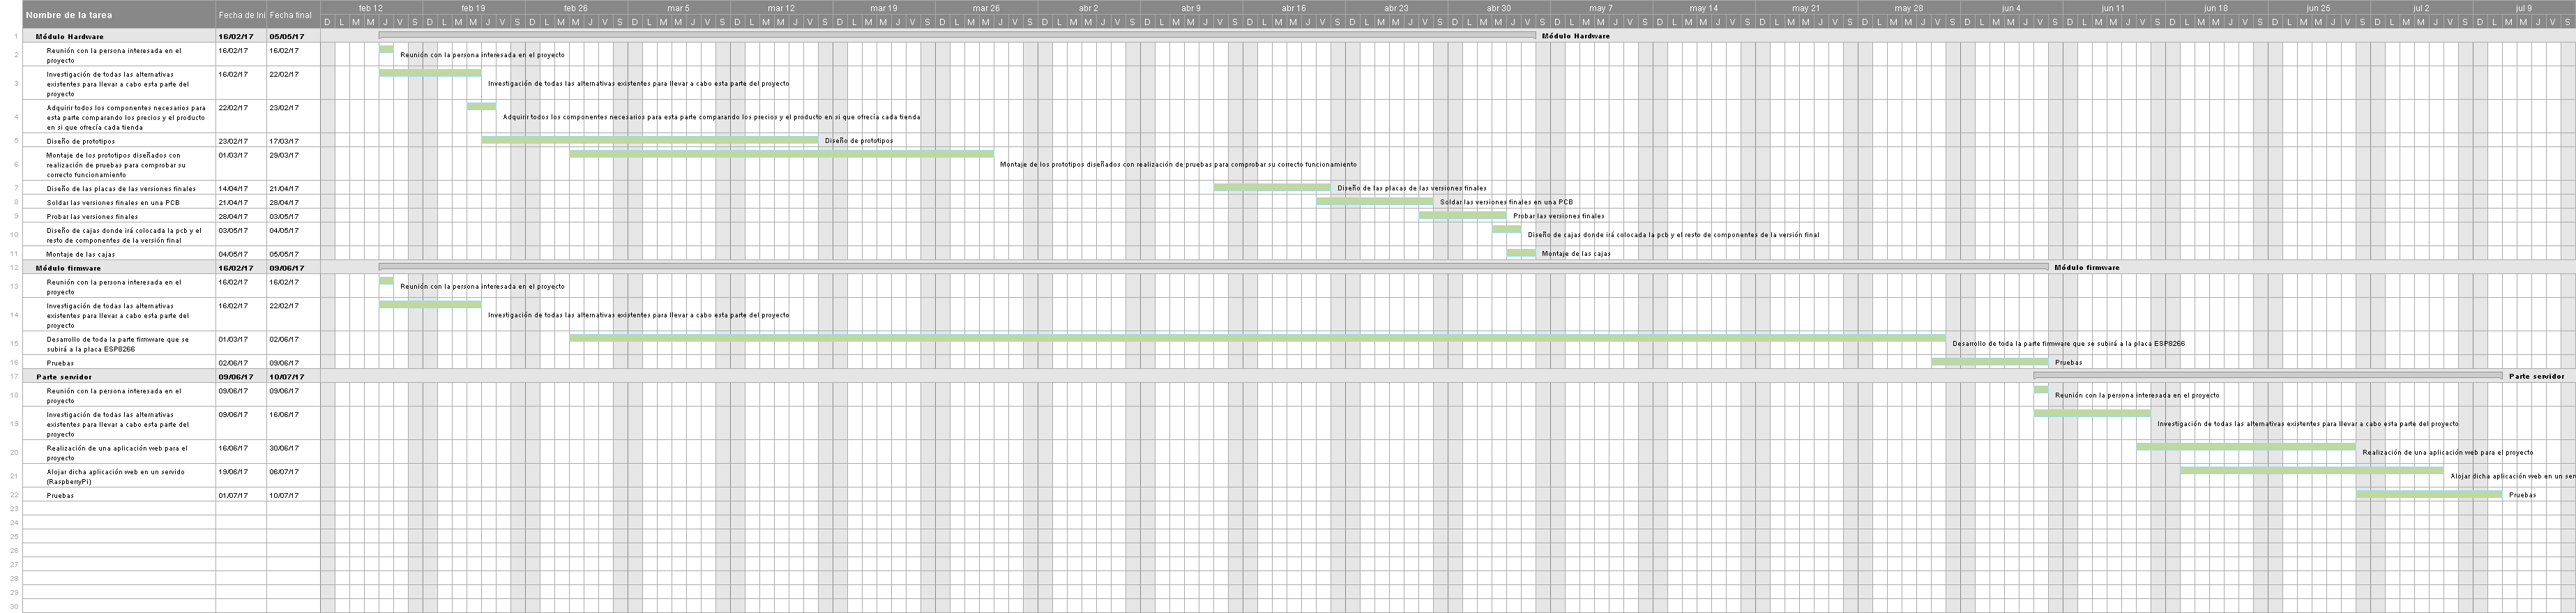
\includegraphics[scale=0.15]{imagenes/gantt.png}
		\caption{Diagrama de Gantt}
		\label{fig:Diagrama de Gantt}
	\end{figure}
	
\end{landscape}

\section{Presupuesto del proyecto}

A continuación se especificará un presupuesto con los costes del proyecto:

\begin{itemize}
	\item\textbf{Hardware y componentes electrónicos :} En el apartado número 4 se especifica detalladamente el coste de todo el hardware adquirido el cuál se sitúa en los \textbf{\EUR{40.47}}, a este tenemos que sumarle otros \EUR{36.76} ya que algunos de los componentes se compraron más de una vez ya que resultaron dañados mientras se realizaron las pruebas. Obteniendo por lo tanto un coste final de \textbf{\EUR{77.23}}
	
	\item\textbf{Parte servidor :} En esta parte el único coste ha sido la adquisición de una Raspberry Pi ya que el sistema operativo utilizado para la Raspberry tiene una licencia gratuita.Las herramientas de desarrollo utilizadas para esta parte son gratuitas como el editor de textos Atom \cite{atom}. El precio de la Raspberry está en torno a los \textbf{\EUR{39.90}}.
	
	\item\textbf{Parte firmware :} Para el desarrollo de esta parte se ha utilizado únicamente software libre en concreto Arduino IDE \cite{arduinoide}, además de bibliotecas con licencia de software libre, por lo tanto el coste ha sido \textbf{\EUR{0}}.
	
	\item\textbf{Horas de trabajo:} El proyecto en total ha tenido una duración total de 7 meses. Para contar las horas de trabajo vamos a suponer que los fines de semana no se ha trabajado por lo tanto si se cuentan los días laborables desde el 16/02/2017 hasta el 2/09/2017 obtenemos un total de 137 días laborables. Trabajando durante una media de 2 horas diarias para poder compatibilizar estudios y la realización de este proyecto obtenemos un total de 274 horas dedicadas a este proyecto. Suponiendo que cada hora se cobre a \EUR{12.5} obtenemos un total de \textbf{\EUR{3425}}.
	
	\item\textbf{Coste del ordenador utilizado para el desarrollo de este proyecto :} Para calcular este coste calcularemos la depreciación \cite{depreciacion} de este producto partiendo de que el precio base son \EUR{800}, calculamos que el ordenador tendrá aproximadamente una vida útil de 5 años con un valor residual de \EUR{100}. Calculamos la base de amortización $ Base amortizacion = valor inicial - valor residual $    por lo que nos queda un valor residual de \EUR{700}. Dividimos este valor entre la vida útil estimada para este ordenador y nos queda un total de \EUR{140} al año. Durante los 7 meses que ha durado este proyecto hemos supuesto que el tiempo que el ordenador ha estado siendo usado son unos 2 meses, por lo tanto obtenemos un precio de \textbf{\EUR{23.33}}.
	
	\item\textbf{Total :} Sumando todos los costes tenemos un total de \textbf{\EUR{3565.46}}
	
\end{itemize}